\chapter{Methodology}

This chapter explains the method developed to locate the sensors in a sensor grid, using the information about the locations of the vertices of the grid and data obtained from the sensors. Before we explain the method we introduce the definitions of the terms that 
are used to explain the method.\\
\begin{definition}{Neighboring sensors:}
 Two sensors are said to be neighbors if they have overlapping field of view.
\end{definition}
\begin{definition}{Grid Adjacency Matrix:}
 We represent the sensor grid in the form of an adjacency matrix. Two vertices of the grid i and j are adjacent if the distance between them ($d_{i,j}$) is less than twice the radius(r) of the sensors field of view.

\[
GAM_{i,j} = 
\begin{cases}
1, &\text{ if } d_{i,j} < \text{  2r } \forall \text{ } i \ne j\\
0, & \text{otherwise}\\
\end{cases}
	\]
From the definitions we can say that neighboring sensors will always be placed on neighboring vertices. 
\end{definition}
Consider a m $\times$ n grid as shown in the figure \ref{fig:Grid}. There are $N= (m\times n)!$ ways in which the sensors can be uniquely placed on the grid. Out of this N ways we have to find out the actual arrangement of the sensors in the grid.  Along with the information of the vertex locations we also have the data from the sensors available. With the help of sensor data we need to determine the sensor location.\\
As neighboring sensors have an overlapping field of view they observe the same events and thus are highly correlated.
On the raw signals of the PIR data stream we use a sliding window with 50\% overlap and calculate the energy using the equation \ref{eq:energyEq}

\begin{equation}
\label{eq:energyEq}
E_s = {\sum_{n=0}^{k}{|x(n)|}^2}
\end{equation}

\begin{figure}
\begin{tikzpicture}
\draw(0,0) node[circle,fill=black]{};
\draw(1.5,0) node[circle,fill=black]{};

\draw(0,2) node[circle,fill=black]{};
\draw(1.5,2) node[circle,fill=black]{};
\draw(0,3.5) node[circle,fill=black]{};
\draw(1.5,3.5) node[circle,fill=black]{};
\foreach \x in {0,1.5,2,2.5,3,3.5,4}
    \foreach \y in {0.5,1,1.5} 
  {
       \node [fill,circle,scale=0.3]  (\x\y) at (\x,\y) {};} 
\draw(4,0) node[circle,fill=black]{};
\draw(4,2) node[circle,fill=black]{};
\draw(4,3.5) node[circle,fill=black]{};
\foreach \x in {2,2.5,3,3.5}
    \foreach \y in {0,0.5,1,1.5,2,3.5} 
  {
       \node [fill,circle,scale=0.3]  (\x\y) at (\x,\y) {};} 
       
       \draw[thick](0,3.5) circle(1cm);
       \draw[|->|, rotate around with nodes={90:(0,3.5)}]
       (0,3.5)--(1,3.5) node[midway,fill=white,rotate with]{r};
       \draw[|<->|](0,3.5)--(1.5,3.5) node[midway,fill=white]{d};
       \draw[thick](1.5,3.5) circle(1cm);
       
\draw [decorate,decoration={brace,amplitude=10pt},xshift=-4pt,yshift=0pt]
(-0.5,0) -- (-0.5,3.5) node [black,midway,xshift=-0.6cm] 
{\footnotesize $M$};

\draw [decorate,decoration={brace,mirror,amplitude=10pt},xshift=-1em,yshift=-2em](0,-0.3) -- (4.5,-0.3) node [black,midway,yshift=-0.6cm]{\footnotesize N};


\end{tikzpicture}
\centering
\caption{A M $\times$ N grid having a sensor with field of view r and distance between the nodes being d.}
\label{fig:Grid}
\end{figure}



With the newly computed energy data stream, compute the cross correlation between all the sensors using equation \ref{eq:corrcoeff}
\begin{equation}
\label{eq:corrcoeff}
r(x,y)=\frac{\sum_{i=1}^{n}(X_i-\overline{X})(Y_i-\overline{Y})}{\sqrt{\sum_{i=1}^{n}(X_i-\overline{X})^2}\sqrt{\sum_{i=1}^{n}(Y_i-\overline{Y})^2}} \\
\end{equation}
X and Y are sensor data stream for sensor X and Y.\\
$\overline{X}$ and $\overline{Y}$ is the mean value of X and Y respectively.\\
n is the number of samples.\\



\begin{figure}
\begin{floatrow}
\ffigbox{
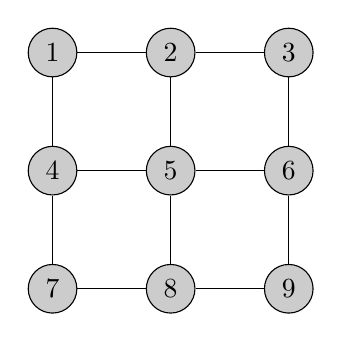
\begin{tikzpicture}[darkstyle/.style={circle,draw,fill=gray!40,minimum size=5}]
\foreach \y in {0,1,2}
 \foreach \x in {0,1,2}
{\pgfmathtruncatemacro{\label}{\x-3*\y+7}
\node[darkstyle](\x\y) at (1.5*\x,1.5*\y){\label};
}
 \foreach \x in {0,1,2}
    \foreach \y [count=\yi] in {0,1}  
      \draw (\x\y)--(\x\yi) (\y\x)--(\yi\x) ;

\end{tikzpicture}

\caption{Correct arrangement}
\label{fig:arrangement1}
}

\ffigbox{
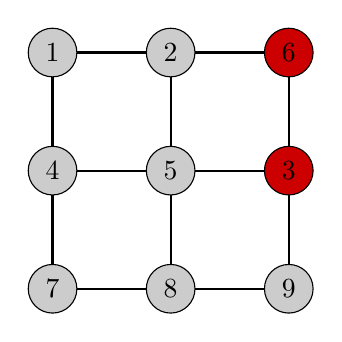
\begin{tikzpicture}[darkstyle/.style={circle,draw,fill=gray!40,minimum size=5}]

\draw[step = 1.5,thick ] (7.4,0) grid (10.5,3);
\node[circle,draw=black,fill=white!80!black,minimum size=5] (7) at (7.5,0) {7};
\node[circle,draw=black,fill=white!80!black,minimum size=5] (4) at (7.5,1.5) {4};
\node[circle,draw=black,fill=white!80!black,minimum size=5] (1) at (7.5,3) {1};

\node[circle,draw=black,fill=white!80!black,minimum size=5] (8) at (9,0) {8};
\node[circle,draw=black,fill=white!80!black,minimum size=5] (5) at (9,1.5) {5};
\node[circle,draw=black,fill=white!80!black,minimum size=5] (2) at (9,3) {2};

\node[circle,draw=black,fill=white!80!black,minimum size=5] (9) at (10.5,0) {9};
\node[circle,draw=black,fill=red!80!black,minimum size=5] (3) at (10.5,1.5) {3};
\node[circle,draw=black,fill=red!80!black,minimum size=5] (6) at (10.5,3) {6};
%\draw [<->,red] (3.east) to [out=60,in=60] (6.east);

\end{tikzpicture}

\caption{Incorrect arrangement}
\label{fig:arrangement2}
}
\centering

\end{floatrow}
\end{figure}


\section{Grid Correlation Sum}
\label{sec:gcs}
Using the cross correlation values between the sensors, we compute correlation matrix R between the n sensor nodes as shown in the equation \ref{eq:corrMatrix} .
\begin{equation}
\label{eq:corrMatrix}
\centering
R = 
\begin{bmatrix}
    r(1,1) & r(1,2) & \dots  & r(1,n) \\
    r(2,1) & r(2,2)  & \dots  & r(2,n) \\
    \vdots & \vdots  & \ddots & \vdots \\
    r(n,1) & r(n,2)  & \dots  & r(n,n)
\end{bmatrix}
\end{equation}\\
r($\alpha$,$\beta$) representing correlation value between the sensor $\alpha$ and $\beta$.\\

Using correlation matrix(R) and grid adjacency matrix(GAM) we define a parameter called \textbf{Grid Correlation Sum (GCS)} as given in the equation \ref{eq:gridCorrelationSum}. 
As the matrices are symmetric along the diagonals we only consider the product of the upper triangle of the matrices.

\begin{equation}
\centering
\text{GCS}=\sum_{i=1}^{n-1}\sum_{j=i+1}^{n}\text{R}(\phi(i),\phi(j))  \times \text{ GAM(i,j)}
\label{eq:gridCorrelationSum}
\end{equation}
\textbf{i,j} represent $ i^{th}$ and $ j^{th}$ vertex on the grid.\\
\textbf{$\phi(i)$} represents the sensor on vertex i.\\
\textbf{R(a,b)}: correlation coefficient between the sensor a and b.\\
\textbf{Grid Adjacency Matrix:}  Adjacency matrix of the grid as definition.\\

We use GCS parameter to identify the correct arrangement out of all the possible arrangement. If we compute  GCS for all the possible arrangements, the one with the maximum correlation sum will represent the actual arrangement of the sensors on the grid.  
If two non neighboring sensors are kept on neighboring vertex or vice versa then the correlation value between those two sensors will be low and thus decreasing the overall sum of the correlation over the grid.
For example Consider the arrangement of the sensor grid in the figure \ref{fig:arrangement1}.
 It consists of 3 $\times$ 3 grid.  
GCS for the  the grid is :\\
\begin{equation*}
GCS_{1}=\text{r(1,2)+ r(1,4)+...r(3,2)+...r(5,6)+...r(8,9)}
\end{equation*}

Now consider the arrangement shown in figure \ref{fig:arrangement2}, where the position of the sensor 3 and 6 are interchanged\\
\begin{equation*}
GCS_{2}=\text{ r(1,2)+r(1,4)+...r(6,2)+...r(3,5)+...r(8,9)}
\end{equation*}

GCS$_{1}$ will be greater than GCS$_{2}$ as r(2,3) $>$ r(2,6) and r(5,6)$>$r(5,3) as sensors 2,6 and 3,5 are non neighboring sensor nodes.\\
When the number of sensors is low we can compute the correct mapping by checking the sum of correlation value for the grid for all the possible N ways. As the number of sensors increase the possible mappings to be checked also increases. We need to find a way to decrease the possible mappings.

\section{Maximum spanning Tree}
Having established a method to determine the true arrangement of the sensor nodes on the grid from all the possible \textbf{N} arrangements, the next step is to prune the possible arrangements. \\
From the definitions of neighboring sensors and neighboring vertices we can say that two neighboring sensors will always be placed on the neighboring vertices. From the grid adjacency matrix we can determine the neighboring vertices of a vertex. If we can determine the neighboring sensor nodes then we can prune the number of possible arrangements by using the constraints that only neighboring sensors can occupy the neighboring vertices. 




%If the neighbors of a sensor are known , the sensors occupying the neighboring vertices on the grid has to be occupied by it's neighboring sensors .
%The neighboring vertices of a vertex \textbf{i} on which a sensor \textbf{a} is located should be occupied by the neighbors of sensor \textbf{a}.
%Thus resulting in the reduction of the number of possible arrangements.

%If we know which are all the neighbors of a sensor then when a sensor is placed on the vertex of a sensor, we know that the neighboring vertex on the grid should only be occupied by it's neighboring nodes. 

Though the correlation value between two neighboring nodes are high compared to the correlation value between the non neighboring nodes, finding a threshold to differentiate between the neighboring and non neighboring nodes when the arrangement is not known is non trivial.\\
Although we might not be able to identify all the neighboring nodes even if we are able to find a minimum of one neighboring node per node we will be able to reduce the number of mappings that needs to be checked. To achieve this we calculate the maximum spanning tree for the correlation matrix \textbf{R}.

If we consider R as an adjacency matrix with each sensor representing a vertex and the correlation value between the sensors representing the edge weight between them. Then the maximum spanning tree for such a graph will connect all the vertices together such that the total weight for the edges in the tree is maximum. The important property of the maximum spanning tree is that 
\begin{itemize}
\item Covers all the sensor nodes
\item It connects a node to another node with which it has the maximum correlation coefficient value.
\end{itemize}


Computing the maximum spanning tree has an edge between 2 nodes which have high correlation matrix compared with the other nodes. Therefore if an edge exists between two nodes in the maximum spanning tree then we can say that those two nodes are neighboring nodes.\\
To compute the maximum spanning tree we use Prim's algorithm \cite{BLTJ:BLTJ1515}.Originally  Prim's algorithm is designed to compute the minimum spanning tree for a graph. In order to compute the maximum spanning tree the correlation matrix is negated and given as the input to the algorithm. The minimum spanning tree obtained from negated weights is the maximum spanning tree for the original weights.This maximum spanning tree represents one of the spanning tree for the grid as can be seen from the figure \ref{fig:MST}. 

\begin{figure}
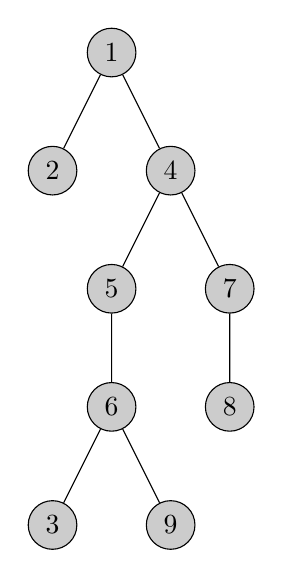
\begin{tikzpicture}[darkstyle/.style={circle,draw,fill=gray!40,minimum size=5}]
\node[darkstyle]{1}
	child{node[darkstyle]{2}}
    child{node[darkstyle]{4}
    	child{node[darkstyle]{5}
	        child{node[darkstyle]{6}
            	child{node[darkstyle]{3}}
                child{node[darkstyle]{9}}}}
                child{node[darkstyle]{7}
                child{node[darkstyle]{8}}}};
\end{tikzpicture}
\qquad \qquad \qquad
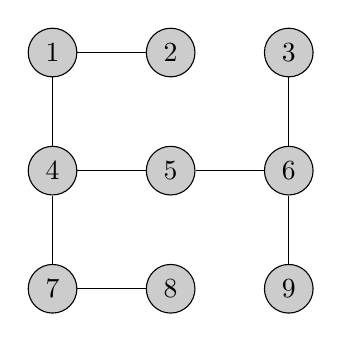
\begin{tikzpicture}[darkstyle/.style={circle,draw,fill=gray!40,minimum size=5}]
\foreach \y in {0,1,2}
 \foreach \x in {0,1,2}
{\pgfmathtruncatemacro{\label}{\x-3*\y+7}
\node[darkstyle](\x\y) at (1.5*\x,1.5*\y){\label};
}
\draw (01)--(02) (02)--(12) (01)--(11) (11)--(21) (21)--(22)
(21)--(20) (00)--(01) (00)--(10);


\end{tikzpicture}
\caption{A maximum spanning tree incident on the grid}
\label{fig:MST}
\end{figure}

\begin{figure}

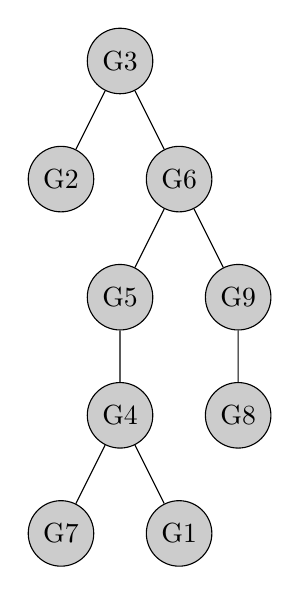
\begin{tikzpicture}[darkstyle/.style={circle,draw,fill=gray!40,minimum size=5}]
\node[darkstyle]{G3}
	child{node[darkstyle]{G2}}
    child{node[darkstyle]{G6}
    	child{node[darkstyle]{G5}
	        child{node[darkstyle]{G4}
            	child{node[darkstyle]{G7}}
                child{node[darkstyle]{G1}}}}
                child{node[darkstyle]{G9}
                child{node[darkstyle]{G8}}}};
\end{tikzpicture}
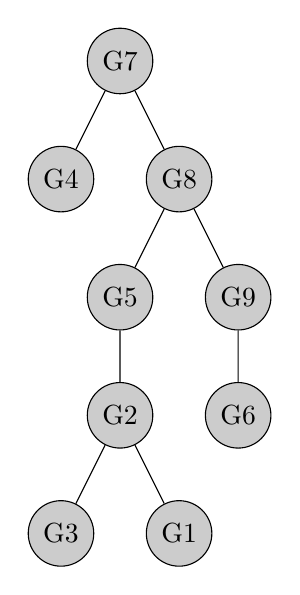
\begin{tikzpicture}[darkstyle/.style={circle,draw,fill=gray!40,minimum size=5}]
\node[darkstyle]{G7}
	child{node[darkstyle]{G4}}
    child{node[darkstyle]{G8}
    	child{node[darkstyle]{G5}
	        child{node[darkstyle]{G2}
            	child{node[darkstyle]{G3}}
                child{node[darkstyle]{G1}}}}
                child{node[darkstyle]{G9}
                child{node[darkstyle]{G6}}}};
\end{tikzpicture}
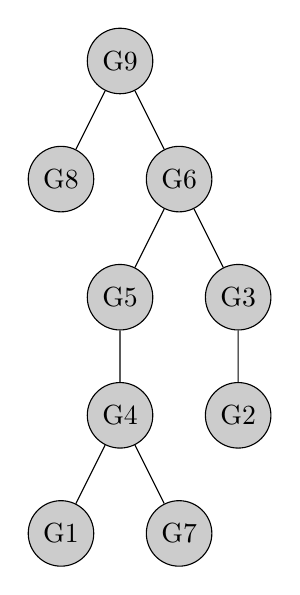
\begin{tikzpicture}[darkstyle/.style={circle,draw,fill=gray!40,minimum size=5}]
\node[darkstyle]{G9}
	child{node[darkstyle]{G8}}
    child{node[darkstyle]{G6}
    	child{node[darkstyle]{G5}
	        child{node[darkstyle]{G4}
            	child{node[darkstyle]{G1}}
                child{node[darkstyle]{G7}}}}
                child{node[darkstyle]{G3}
                child{node[darkstyle]{G2}}}};
\end{tikzpicture}
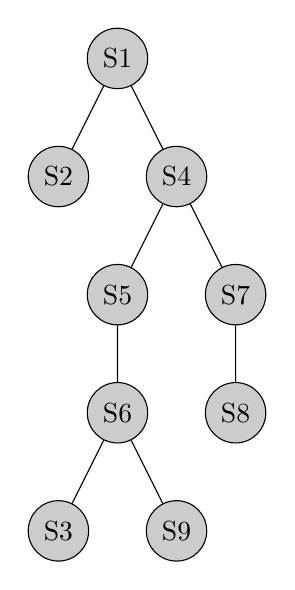
\begin{tikzpicture}[darkstyle/.style={circle,draw,fill=gray!40,minimum size=5}]
\node[darkstyle]{S1}
	child{node[darkstyle]{S2}}
    child{node[darkstyle]{S4}
    	child{node[darkstyle]{S5}
	        child{node[darkstyle]{S6}
            	child{node[darkstyle]{S3}}
                child{node[darkstyle]{S9}}}}
                child{node[darkstyle]{S7}
                child{node[darkstyle]{S8}}}};
\end{tikzpicture}
\end{figure}







\begin{figure}
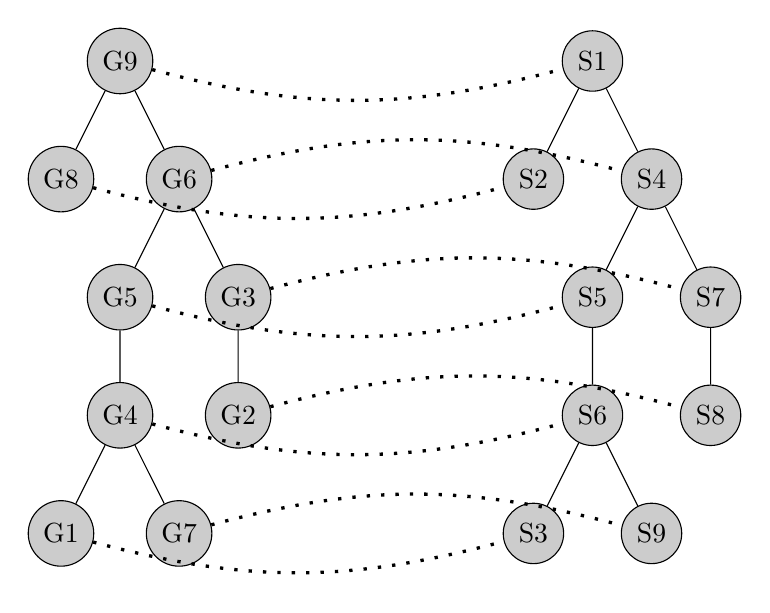
\begin{tikzpicture}[darkstyle/.style={circle,draw,fill=gray!40,minimum size=5}]
\begin{scope}
\node[darkstyle](G9){G9}
	child{node[darkstyle](G8){G8}}
    child{node[darkstyle](G6){G6}
    	child{node[darkstyle](G5){G5}
	        child{node[darkstyle](G4){G4}
            	child{node[darkstyle](G1){G1}}
                child{node[darkstyle](G7){G7}}}}
                child{node[darkstyle](G3){G3}
                child{node[darkstyle](G2){G2}}}};
\end{scope}
\qquad
\begin{scope}[shift={(6,0)}]
\node[darkstyle](S1){S1}
	child{node[darkstyle](S2){S2}}
    child{node[darkstyle](S4){S4}
    	child{node[darkstyle](S5){S5}
	        child{node[darkstyle](S6){S6}
            	child{node[darkstyle](S3){S3}}
                child{node[darkstyle](S9){S9}}}}
                child{node[darkstyle](S7){S7}
                child{node[darkstyle](S8){S8}}}};
\end{scope}
\draw[loosely dotted,very thick] (G9)to[out=0-15,in=195](S1);
\draw[loosely dotted,very thick] (G8)to[out=0-15,in=195](S2);
\draw[loosely dotted,very thick] (G6)to[out=15,in=165](S4);
\draw[loosely dotted,very thick] (G5)to[out=0-15,in=195](S5);
\draw[loosely dotted,very thick] (G4)to[out=0-15,in=195](S6);
\draw[loosely dotted,very thick] (G1)to[out=0-15,in=195](S3);
\draw[loosely dotted,very thick] (G7)to[out=15,in=165](S9);
\draw[loosely dotted,very thick] (G3)to[out=15,in=165](S7);
\draw[loosely dotted,very thick] (G2)to[out=15,in=165](S8);
\end{tikzpicture}

\end{figure}

% Graph monomorphism 

\section{Graph Monomorphism} 

In the previous section we obtain a maximum spanning tree for the correlation matrix and saw how this represents a spanning tree for the grid. In this section we describe how to obtain the sensor location on the grid using the maximum spanning tree.
We can classify the problem of obtaining the mapping between a spanning tree of a graph G to itself as a problem of graph Monomorphism. 

% Monomorphism problem
Let us consider a base graph G(M,A) and a pattern graph H(N,B) with vertex set M,N and edge set A and B respectively. A problem of finding all the Monomorphisms of the pattern graph into the base graph is defined as Monomorphism problem.

Two graphs 
 $G =( V_G, E_G)$ and
 H =$( V_H, E_H)$  are monomorphic  if and only if there exists an injective (node)
mapping $\phi V_G \rightarrow  V_H$ : for which $\forall v,w \in V_G:(v,w) \in E_G \Rightarrow (\phi((v),\space \phi(w)) \in E_H.$\\  holds
true. 

Monomorphism is often confused with subgraph isomorphism. Monomorphism is weaker kind of subgraph Monomorphism. \\
Two graphs  $G =( V_G, E_G)$ and
 H =$( V_H, E_H)$  are sub graph isomorphic  if and only if there exists an injective (node)
mapping $\phi( V_G) \rightarrow  V_H$ : for which $\forall v,w \in V_G:(v,w) \in E_G \Leftrightarrow (\phi((v),\space \phi(w)) \in E_H.$\\  holds
true. 
The relationship between edges of the graphs are equivalence for subgraph isomorphism, and for Monomorphism  relationship  is an implication. It is well known that Graph Monomorphism is a
well NP-Complete problem \cite{Garey:1979:CIG:578533}. As discussed in section \ref{LitReview} there have been several algorithms that have been proposed to solve the problem of Monomorphism.
In our work we make use of the VF2 algorithm.


\subsection{VF2}

In this section we give a brief description about VF2 algorithm.\\
Pseudo-code \\
\begin{figure}

\begin{algorithm}[H]
\begin{algorithmic}
 \LState  \textbf{Procedure} Match(s)\\
\textbf{INPUT:}  an intermediate state s; the initial state $s_0$ has $M(s_0)=\emptyset$\\
\textbf{OUTPUT:} the mappings between two graphs>\;
\textbf{Match(s)}\\
 \textbf{IF} M(s) covers all the nodes of $G_2$ \textbf{THEN}\\
               \textbf{OUTPUT} M(s)\\
\textbf{ELSE}\\
                 Compute the set P(s) of the pairs of candidates for inclusion in M(s)\\
\textbf{FOREACH} (n,m) $\in$ P(s)\\
\textbf{IF} F(s,n,m) \textbf{THEN}\\
	Compute the state s' obtained by adding (n,m) to M(s)\\
\textbf{CALL} Match(s')\\
\textbf{ENDIF}\\
\textbf{ENDFOREACH}\\
Restore data structure\\
\textbf{ENDIF}\\

\end{algorithmic}
\end{algorithm}
\caption{Pseudo code for VF2 algorithm}
\label{fig:VF2}
\end{figure}
Consider the graphs shown in figure \ref{fig:gridTree} representing 

% VF2 explanation 
VF2 algorithm is an algorithm to solve subgraph isomorphism problem. VF2 is a depth search first algorithm. It uses recursive backtracking technique. A process of matching 
the grid graph G to its spanning tree consists of determining a mapping M which associate nodes of $Grid(G)$ with nodes of the Tree(T) and vice versa, with some constraints.
Mapping is expressed as a set of pairs (n,m) with (n $\in$ G and m $\in$ T). 
In VF2 algorithm the process of finding a mapping is represented as a State Space Representation (SSR). Each state s of the matching process can be associated to a partial mapping solution M(s),
which contains only a subset of M. A transition from current state(s) to the next state(s') represents the addition of a mapping (n,m) to the state s.

VF2 algorithm introduces a set of rules which helps to prune the number of possible SSR that needs to be checked before obtaining the a valid mapping. Figure \ref{fig:VF2} gives a high-lvel description of the VF2 algorithm.
There are 2 important functionalities in the algorithm one is the generation of possible mappings and the other is the checking of the validity of the mapping.

\subsection{Computation of candidate pair set P(s)}
This section explains the method to compute the candidate pair set P(S) for an undirected graph G and T. 
Set $T_1(s)$ and $T_2(s)$ are defined for Graph G and T respectively, representing the nodes which are neighbors of the set of nodes including in the partial mapping state(s).
Set P(s) will be made of all the the node pairs(n,m) with n$\in$ G and m $\in$ T. If either of $T_1$ or $T_2$ set is empty then the set P(s) will the pair of nodes not contained in either G(s) or T(s).
\subsection{Feasibility Rules}
Feasibility Rules are used to check the consistency of the partial solution s' obtained by adding nodes n,m and prune the search tree. The functionality of the rules are as explained below.
Gata graph (G), Querry graph(Q)
In vf2 algorithm, those candidates(m,n) are pruned if m is not connected to already matched nodes in $G_q$
(i.e nodes of $G_q$ included in M).
Subsequently, the pruning step also removes those node-pairs(m,n) in which n is not connected to the matched 
nodes in the data Graph G. These pruning rules assume that the query and data graph are connected.

The algorithm also compares the number of neighboring nodes of each n and m that are connected to nodes in M but are not
included in M. The number of such nodes in the data graph must be greater than or equal to the number of such nodes in the query graph.
finally the number of neighbors nodes of each of n and iq that are not directly connected to nodes in M are compared. The number of 
such nodes in the data graph must be no smaller than the number of such nodes in the query graph.

\section{Determination of sensor placement}
After we obtain the various mappings. We need to decide which out of the various mappings gives the actual placement of the sensors on the grid. To identify the correct mapping we compute GCS as explained in section \ref{sec:gcs}. We calculate the grid correlation sum for all the mappings obtained and the mappings which gives the maximum sum will be the actual placement of the sensors on the grid.





 






 


